% =====================================================================
%  TRABAJO PARCIAL --- ROBÓTICA Y SISTEMAS AUTÓNOMOS 2026-2
%  Robot Antropomórfico de 3 GDL (RRR)
%  Autores: Amit Roy Flores Rivera, Franklin Enrique Alegría Barboza,
%           José Luis Espinoza Chamaya, Raquel Medianero, Yasmín Urrego
%  Docente: Ing. Wilson Dennis Reyes Vásquez
%  UNI --- Facultad de Ingeniería Industrial y de Sistemas --- Posgrado
% =====================================================================
\documentclass[11pt,a4paper]{article}

% ---------- Paquetes esenciales ----------
\usepackage[utf8]{inputenc}
\usepackage[T1]{fontenc}
\usepackage{amsmath,amssymb,amsthm,mathtools}
\usepackage{bm}
\usepackage{geometry}
\geometry{a4paper, top=2.4cm, bottom=2.4cm, left=2.3cm, right=2.3cm}
\usepackage{graphicx}
\usepackage{booktabs}
\usepackage{tabularx}
\usepackage{array}
\usepackage{multirow}
\usepackage{xcolor}
\usepackage{tcolorbox}
\tcbuselibrary{skins,breakable}
\usepackage{enumitem}
\usepackage{caption}
\usepackage{subcaption}
\usepackage{listings}
\usepackage{tikz}
\usetikzlibrary{arrows.meta,positioning,calc,shapes.geometric,fit,backgrounds}

% ---------- Idioma español ----------
\renewcommand{\contentsname}{Índice General}
\renewcommand{\listfigurename}{Índice de Figuras}
\renewcommand{\listtablename}{Índice de Tablas}
\renewcommand{\figurename}{Figura}
\renewcommand{\tablename}{Tabla}
\renewcommand{\refname}{Referencias bibliográficas (Norma APA 7.ª ed.)}
\renewcommand{\abstractname}{Resumen Ejecutivo}
\renewcommand{\appendixname}{Anexos}

\usepackage[colorlinks=true,
  linkcolor=blue!60!black,
  citecolor=teal!50!black,
  urlcolor=blue!70!black,
  bookmarks=true,
  bookmarksnumbered=true,
  pdftitle={Trabajo Parcial --- Robot Antropomórfico de 3 GDL},
  pdfauthor={A. Flores, F. Alegría, J. Espinoza, R. Medianero, Y. Urrego},
  pdfsubject={Robótica y Sistemas Autónomos UNI 2026-2},
  pdfkeywords={Robot 3GDL, Denavit-Hartenberg, Jacobiano Geométrico, Singularidades, CLIK-DLS, CTC, NSGA-II, MPC, MuJoCo, MATLAB}
]{hyperref}
\captionsetup{font=small,labelfont=bf,labelsep=period}

% ---------- Colores institucionales UNI ----------
\definecolor{uniGranate}{HTML}{7A121C}
\definecolor{uniAzul}{HTML}{0B2447}
\definecolor{uniAzulC}{HTML}{1F6FEB}
\definecolor{uniRojo}{HTML}{B01818}
\definecolor{uniOro}{HTML}{C59B27}
\definecolor{cajaBg}{HTML}{F4F8FD}
\definecolor{cajaBorde}{HTML}{1F6FEB}
\definecolor{codigoBg}{HTML}{F4F6F9}
\definecolor{verdeOk}{HTML}{1B8E3A}
\definecolor{naranja}{HTML}{C97A0A}

% ---------- Cajas tipo callout ----------
\newtcolorbox{cajadef}[1][]{%
  enhanced,
  colback=cajaBg, colframe=cajaBorde,
  boxrule=0.6pt, arc=2pt,
  left=10pt, right=10pt, top=6pt, bottom=6pt,
  fonttitle=\bfseries\color{white},
  coltitle=white, colbacktitle=cajaBorde,
  title={#1}}

\newtcolorbox{cajaidea}[1][]{%
  enhanced,
  colback=green!5!white, colframe=verdeOk,
  boxrule=0.6pt, arc=2pt,
  left=10pt, right=10pt, top=6pt, bottom=6pt,
  fonttitle=\bfseries\color{white},
  coltitle=white, colbacktitle=verdeOk,
  title={#1}}

\newtcolorbox{cajaadv}[1][]{%
  enhanced,
  colback=orange!8!white, colframe=naranja,
  boxrule=0.6pt, arc=2pt,
  left=10pt, right=10pt, top=6pt, bottom=6pt,
  fonttitle=\bfseries\color{white},
  coltitle=white, colbacktitle=naranja,
  title={#1}}

% ---------- Listings MATLAB ----------
\lstdefinestyle{matlabstyle}{
  language=Matlab,
  basicstyle=\ttfamily\scriptsize,
  keywordstyle=\color{uniAzulC}\bfseries,
  commentstyle=\color{gray}\itshape,
  stringstyle=\color{verdeOk},
  numbers=left, numberstyle=\tiny\color{gray},
  numbersep=6pt,
  backgroundcolor=\color{codigoBg},
  frame=single, framerule=0.3pt, rulecolor=\color{gray!40},
  tabsize=2, showstringspaces=false, breaklines=true,
  captionpos=b,
  literate={á}{{\'a}}1 {é}{{\'e}}1 {í}{{\'i}}1 {ó}{{\'o}}1 {ú}{{\'u}}1 {ñ}{{\~n}}1 {º}{{\textdegree}}1
}
\lstset{style=matlabstyle}

% ---------- Comandos abreviados ----------
\newcommand{\Real}{\mathbb{R}}
\newcommand{\T}{^{\!\top}}
\newcommand{\norm}[1]{\left\lVert#1\right\rVert}
\newcommand{\abs}[1]{\left\lvert#1\right\rvert}
\newcommand{\qdot}{\dot{\bm{q}}}
\newcommand{\qddot}{\ddot{\bm{q}}}
\newcommand{\pdot}{\dot{\bm{p}}}
\newcommand{\Jdls}{J^{\dagger}_{\text{\tiny DLS}}}

% ---------- Encabezado y pie ----------
\usepackage{fancyhdr}
\setlength{\headheight}{14pt}
\pagestyle{fancy}
\fancyhf{}
\fancyhead[L]{\small\itshape Trabajo Parcial --- Robot Antropomórfico de 3 GDL}
\fancyhead[R]{\small\textsc{UNI --- Posgrado FIIS 2026-2}}
\fancyfoot[C]{\small\thepage}
\renewcommand{\headrulewidth}{0.4pt}
\renewcommand{\footrulewidth}{0pt}

\widowpenalty=10000
\clubpenalty=10000
\tolerance=1800
\emergencystretch=20pt
\hyphenpenalty=100

% =====================================================================
\begin{document}

% ---------- 1. CARÁTULA OFICIAL UNI ----------
\begin{titlepage}
\thispagestyle{empty}
\centering
{\color{uniGranate}\rule{\textwidth}{2.8pt}}\\[4mm]

% DESPUÉS (logo real):
% Escudo institucional oficial de la UNI (logo.jpeg)

\includegraphics[width=4.2cm, keepaspectratio]{logo.jpeg}\\[3mm]

{\Large\bfseries\scshape\color{uniGranate} Universidad Nacional de Ingeniería}\\[1.5mm]
{\normalsize\bfseries Facultad de Ingeniería Industrial y de Sistemas}\\
{\normalsize Unidad de Posgrado}\\[5mm]
{\large\bfseries\color{uniAzul} MAESTRÍA EN INGENIERÍA DE SISTEMAS / INTELIGENCIA ARTIFICIAL}\\
{\normalsize Asignatura: Robótica y Sistemas Autónomos}\\[8mm]

{\color{uniAzul}\rule{0.82\textwidth}{0.8pt}}\\[5mm]
{\LARGE\bfseries\color{uniAzul} «TRABAJO PARCIAL»}\\[4mm]
{\Large\bfseries «Robot Antropomórfico de 3\,GDL»}\\[3mm]
{\normalsize Modelado de la cinemática directa (geométrica, MTH y Denavit-Hartenberg), cinemática inversa de doble rama, cinemática diferencial ($J_{v}$ y $J_{\omega}$), análisis de singularidades, control cinemático CLIK-DLS y control dinámico híbrido evolutivo (CTC / MPC / NSGA-II) con simulación de enceste y cambio de estado en MATLAB y MuJoCo}\\[5mm]
{\color{uniAzul}\rule{0.82\textwidth}{0.8pt}}\\[10mm]

\begin{tabular}{>{\raggedleft\arraybackslash}p{3.8cm} p{8.8cm}}
\textbf{Curso:}          & Robótica y Sistemas Autónomos\\[2mm]
\textbf{Docente:}        & Ing. Wilson Dennis Reyes Vásquez\\[2mm]
\textbf{Semestre:}       & Académico 2026\,--\,2\\[2mm]
\textbf{Autores:}        & Flores Rivera, Amit Roy\\
                         & Alegría Barboza, Franklin Enrique\\
                         & Espinoza Chamaya, José Luis\\
                         & Medianero Huari, Raquel\\
                         & Urrego Montoya, Yasmín Mariela\\[2mm]
\textbf{Caso de estudio:}& Manipulador Antropomórfico RRR de 3\,GDL (Conejo Benítez, 2021)\\
\end{tabular}

\vfill
{\small\textsc{Lima, Perú --- 2026}}\\[2mm]
{\color{uniGranate}\rule{\textwidth}{2.8pt}}
\end{titlepage}

% ---------- ÍNDICE ----------
\tableofcontents
\newpage

% =====================================================================
\section{Introducción}
% =====================================================================

El modelado matemático y el control de movimiento de manipuladores robóticos antropomórficos de tres grados de libertad (3\,GDL, configuración rotacional RRR) constituyen la base fundamental para el diseño de sistemas autónomos de manipulación industrial, quirúrgica y de servicio. A diferencia de los servomecanismos lineales desacoplados, un manipulador antropomórfico espacial exhibe fuertes acoplamientos inerciales no lineales entre eslabones, fuerzas centrífugas y de Coriolis dependientes del producto de velocidades articulares, pares gravitacionales variables con la postura y configuraciones singulares donde la matriz Jacobiana pierde rango (Barrientos et~al., 2007; Craig, 2018; Siciliano et~al., 2009).

En cumplimiento de las pautas del Trabajo Parcial de la asignatura \emph{Robótica y Sistemas Autónomos} (Ciclo 2026-2), en el presente informe se desarrolla el análisis exhaustivo y la simulación computacional de la \textbf{cinemática directa}, \textbf{cinemática inversa}, \textbf{cinemática diferencial}, \textbf{análisis de singularidades} y \textbf{control cinemático y dinámico} de un robot antropomórfico real de 3\,GDL tomado de la literatura científica (Conejo Benítez, 2021): altura de base $d_{1}=0{,}079\;\text{m}$, brazo primario $L_{1}=0{,}113\;\text{m}$ y antebrazo-efector $L_{2}=0{,}140\;\text{m}$. La solución se implementa de forma dual y verificada tanto en \textbf{MATLAB} (\texttt{matlab/simulacion\_3gdl\_examen\_parcial.m}, siguiendo la estructura de los ejercicios desarrollados en clase) como en un \textbf{Gemelo Digital 3D interactivo en Python/MuJoCo} (Todorov et~al., 2012) (\texttt{main.py}).

Asimismo, con el objetivo de dotar al manipulador de una aplicación funcional concreta y medible ---evaluando su capacidad para apuntar con precisión milimétrica como una lente óptica focal o encestar una esfera en aros objetivo---, se demuestra desde primeros principios cinemáticos que una cadena RRR de 3\,GDL gobierna las tres coordenadas traslacionales del efector $\bm{p}=[x,y,z]\T\in\Real^{3}$ dentro de una envolvente toroidal-esférica de radio máximo $R_{\max}=L_{1}+L_{2}=0{,}253\;\text{m}$. Sobre esta base se construyó una arquitectura interactiva que integra un \emph{Modo Laboratorio de Lente/Puntero de Precisión} ($<2{,}0\;\text{mm}$) y un \emph{Modo Juego «Circuito de 5 Aros (Encestar Bola)»}, con velocímetro cartesiano en tiempo real $\norm{\pdot}=\norm{J_{v}(\bm{q})\,\qdot}$, registro de velocidad pico $v_{\max}$ y máquina de estados con cambio de color 3D instantáneo cuando el efector encesta o bloquea el objetivo.

Las interrogantes científicas que guían la investigación son:
\begin{enumerate}[label=(\roman*), topsep=3pt, itemsep=2pt]
\item ¿Cómo relacionar y verificar simbólicamente los tres métodos de cinemática directa (geométrico, matrices de transformación homogénea sucesivas y algoritmo de Denavit-Hartenberg) junto con las dos ramas de la cinemática inversa?
\item ¿Cómo caracterizar algebraica y geométricamente el Jacobiano completo $6\times 3$ ($J_{v}$ lineal y $J_{\omega}$ angular) y garantizar el cruce continuo por la singularidad de codo ($\det J_{v}=0$) mediante la pseudoinversa amortiguada de Levenberg--Marquardt (DLS)?
\item ¿En qué medida el control cinemático en lazo cerrado (CLIK-DLS) y la sintonización evolutiva multiobjetivo NSGA-II (Deb et~al., 2002) del control por torque computado (CTC) superan al controlador nominal en error de seguimiento, tiempo de captura y recuperación ante perturbaciones?
\end{enumerate}

% =====================================================================
\section{Desarrollo o cuerpo del trabajo}
% =====================================================================

% ---------------------------------------------------------------------
\subsection{Parámetros físicos, volumen de trabajo y cinemática directa (Geométrica, MTH y Denavit-Hartenberg)}
\label{sec:fk}
% ---------------------------------------------------------------------

El manipulador antropomórfico real estudiado (Conejo Benítez, 2021, Tabla~3.2) está constituido por tres articulaciones rotacionales ($\text{R--R--R}$) accionadas por servomotores Dynamixel (AX-18A en la cintura y AX-12A en hombro y codo):
\begin{itemize}[leftmargin=*, topsep=2pt, itemsep=1pt]
\item \textbf{Articulación 1 ($q_{1}$, cintura/base):} gira alrededor del eje vertical $Z_{0}$ con rango $q_{1}\in[-2{,}80,\;+2{,}80]\;\text{rad}$ y par máximo $\tau_{1,\max}=0{,}70\;\text{N\,m}$ (altura de hombro $d_{1}=0{,}079\;\text{m}$).
\item \textbf{Articulación 2 ($q_{2}$, hombro):} eleva el primer eslabón ($L_{1}=0{,}113\;\text{m}$) respecto al plano horizontal con rango $q_{2}\in[-1{,}25,\;+1{,}35]\;\text{rad}$ y par máximo $\tau_{2,\max}=0{,}70\;\text{N\,m}$.
\item \textbf{Articulación 3 ($q_{3}$, codo):} flexiona el segundo eslabón ($L_{2}=0{,}140\;\text{m}$) con rango $q_{3}\in[-2{,}40,\;+2{,}40]\;\text{rad}$ y par máximo $\tau_{3,\max}=0{,}45\;\text{N\,m}$.
\end{itemize}

Siguiendo la metodología desarrollada en las sesiones prácticas del curso, el modelo cinemático directo se formula y comprueba mediante tres métodos equivalentes:

\paragraph{1. Método del Algoritmo de Denavit-Hartenberg (DH).}
Asignando los sistemas de referencia ortonormales $\{S_{0}\},\{S_{1}\},\{S_{2}\},\{S_{3}\}$ conforme a la Figura~\ref{fig:esquema}, se obtiene la Tabla~\ref{tab:dh} de parámetros de Denavit-Hartenberg estándar.

\begin{table}[htbp]
\centering
\caption{Parámetros de Denavit-Hartenberg estándar del robot antropomórfico RRR de 3\,GDL.}\label{tab:dh}
\small
\begin{tabular}{cccccc}
\toprule
Eslabón $i$ & $\theta_{i}$ (rad) & $d_{i}$ (m) & $a_{i}$ (m) & $\alpha_{i}$ (rad) & Articulación \\
\midrule
1 & $q_{1}$ & $d_{1}=0{,}079$ & $0{,}000$       & $+\pi/2$ & Rotacional ($Z_{0}$ vertical) \\
2 & $q_{2}$ & $0{,}000$       & $L_{1}=0{,}113$ & $0$      & Rotacional ($Z_{1}$ horizontal) \\
3 & $q_{3}$ & $0{,}000$       & $L_{2}=0{,}140$ & $0$      & Rotacional ($Z_{2}\parallel Z_{1}$) \\
\bottomrule
\end{tabular}
\end{table}

\begin{figure}[htbp]
\centering
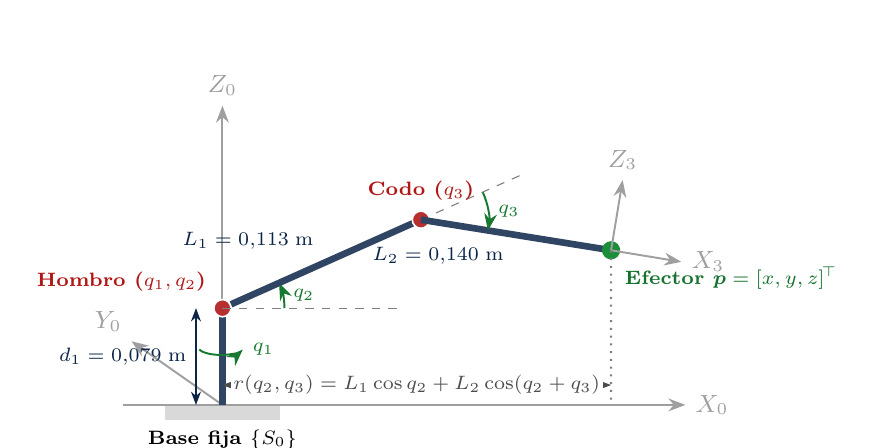
\begin{tikzpicture}[>=Stealth, scale=1.05, font=\small,
   link/.style={line width=2.4pt, draw=uniAzul!85},
   joint/.style={circle, fill=uniRojo!90, draw=white, line width=0.6pt, inner sep=2.2pt},
   axis/.style={->, line width=0.7pt, color=gray!75},
   ang/.style={->, line width=0.7pt, color=verdeOk!85!black}]
% Base
\fill[gray!30] (-0.7,0) rectangle (0.7,0.18);
\draw[thick, uniAzul] (-0.7,0.18) -- (0.7,0.18);
\node[below, font=\scriptsize\bfseries] at (0,0) {Base fija $\{S_0\}$};
% Ejes base X0, Y0, Z0
\draw[axis] (-1.2,0.18) -- (5.6,0.18) node[right] {$X_0$};
\draw[axis] (0,0.18) -- (-1.1,0.95) node[above left] {$Y_0$};
\draw[axis] (0,0.18) -- (0,3.8) node[above] {$Z_0$};
% Columna d1
\draw[link] (0,0.18) -- (0,1.35);
\draw[<->, thin, color=uniAzul] (-0.32,0.18) -- (-0.32,1.35) node[midway, left, font=\scriptsize] {$d_1=0{,}079\;\text{m}$};
% Arco de giro q1 alrededor de Z0
\draw[ang] (-0.28,0.85) arc[start angle=200, end angle=340, x radius=0.28, y radius=0.10] node[right, font=\scriptsize] {$q_1$};
% Nudo Hombro (q1, q2)
\node[joint, label={[font=\scriptsize\bfseries, color=uniRojo]above left:{Hombro ($q_1,q_2$)}}] (sh) at (0,1.35) {};
% Linea horizontal de referencia para q2
\draw[dashed, gray] (0,1.35) -- (2.2,1.35);
\draw[ang] (0.75,1.35) arc[start angle=0, end angle=24, radius=0.75] node[midway, right, font=\scriptsize] {$q_2$};
% Eslabon L1 (inclinado 24 grados)
\coordinate (el) at (2.4,2.42);
\draw[link] (sh) -- (el) node[midway, above left, font=\scriptsize, color=uniAzul] {$L_1=0{,}113\;\text{m}$};
% Linea prolongacion de L1 para mostrar q3
\draw[dashed, gray] (el) -- ($(el)+(1.2,0.535)$);
% Nudo Codo (q3)
\node[joint, label={[font=\scriptsize\bfseries, color=uniRojo]above:{Codo ($q_3$)}}] at (el) {};
% Eslabon L2
\coordinate (ef) at (4.7,2.05);
\draw[link] (el) -- (ef) node[midway, below left, font=\scriptsize, color=uniAzul] {$L_2=0{,}140\;\text{m}$};
\draw[ang] ($(el)+(0.75,0.33)$) arc[start angle=24, end angle=-9, radius=0.82] node[midway, right, font=\scriptsize] {$q_3$};
% Efector final y marco {S3}
\fill[verdeOk] (ef) circle (0.11);
\draw[axis] (ef) -- ($(ef)+(0.85,-0.14)$) node[right] {$X_3$};
\draw[axis] (ef) -- ($(ef)+(0.14,0.85)$) node[above] {$Z_3$};
\node[below right, font=\scriptsize\bfseries, color=verdeOk!80!black] at ($(ef)+(0.05,-0.08)$) {Efector $\bm{p}=[x,y,z]\T$};
% Proyeccion radial r
\draw[dotted, thick, gray] (ef) -- (4.7,0.18);
\draw[<->, thin, color=gray!60!black] (0,0.42) -- (4.7,0.42) node[midway, fill=white, inner sep=1pt, font=\scriptsize] {$r(q_2,q_3) = L_1\cos q_2 + L_2\cos(q_2+q_3)$};
\end{tikzpicture}
\caption{Esquema cinemático tridimensional del manipulador antropomórfico RRR de 3\,GDL con asignación de marcos $\{S_{0}\}\dots\{S_{3}\}$ y variables articulares $(q_{1},q_{2},q_{3})$.}
\label{fig:esquema}
\end{figure}

En coincidencia con la función \texttt{DHL(theta,d,a,alpha)} empleada en las sesiones de laboratorio en MATLAB (\texttt{M = Mrot\_z * transl * Mrot\_x}), cada matriz de transformación homogénea elemental se define como:
\begin{equation}\label{eq:dh}
A_{i}(\theta_{i},d_{i},a_{i},\alpha_{i})=
\operatorname{Rot}_{z}(\theta_{i})\,\operatorname{Trans}(a_{i},0,d_{i})\,\operatorname{Rot}_{x}(\alpha_{i})=
\begin{bmatrix}
\cos\theta_{i} & -\sin\theta_{i}\cos\alpha_{i} &  \sin\theta_{i}\sin\alpha_{i} & a_{i}\cos\theta_{i}\\
\sin\theta_{i} &  \cos\theta_{i}\cos\alpha_{i} & -\cos\theta_{i}\sin\alpha_{i} & a_{i}\sin\theta_{i}\\
0              &  \sin\alpha_{i}              &  \cos\alpha_{i}               & d_{i}\\
0              &  0                            &  0                            & 1
\end{bmatrix}.
\end{equation}

Evaluando~\eqref{eq:dh} para cada fila de la Tabla~\ref{tab:dh} se obtienen las tres matrices individuales explícitas:
{\small\setlength{\arraycolsep}{3.0pt}
\begin{equation}\label{eq:A123}
A_{1}(q_{1})=
\begin{bmatrix}
\cos q_{1} & 0 &  \sin q_{1} & 0\\
\sin q_{1} & 0 & -\cos q_{1} & 0\\
0          & 1 &  0          & d_{1}\\
0          & 0 &  0          & 1
\end{bmatrix},\;\;
A_{2}(q_{2})=
\begin{bmatrix}
\cos q_{2} & -\sin q_{2} & 0 & L_{1}\cos q_{2}\\
\sin q_{2} &  \cos q_{2} & 0 & L_{1}\sin q_{2}\\
0          &  0          & 1 & 0\\
0          &  0          & 0 & 1
\end{bmatrix},\;\;
A_{3}(q_{3})=
\begin{bmatrix}
\cos q_{3} & -\sin q_{3} & 0 & L_{2}\cos q_{3}\\
\sin q_{3} &  \cos q_{3} & 0 & L_{2}\sin q_{3}\\
0          &  0          & 1 & 0\\
0          &  0          & 0 & 1
\end{bmatrix}.
\end{equation}}

Multiplicando en cadena $T_{0}^{3}(\bm{q})=A_{1}(q_{1})\,A_{2}(q_{2})\,A_{3}(q_{3})$ y aplicando las identidades trigonométricas de suma de ángulos ($c_{23}=\cos(q_{2}+q_{3})$, $s_{23}=\sin(q_{2}+q_{3})$), resulta la matriz homogénea total del efector respecto a la base:
\begin{equation}\label{eq:t03}
T_{0}^{3}(\bm{q})=
\begin{bmatrix}
\bm{n}(\bm{q}) & \bm{o}(\bm{q}) & \bm{a}(\bm{q}) & \bm{p}(\bm{q})\\
0 & 0 & 0 & 1
\end{bmatrix}=
\begin{bmatrix}
\cos q_{1}\,c_{23} & -\cos q_{1}\,s_{23} &  \sin q_{1} & \bigl(L_{1}\cos q_{2}+L_{2}\,c_{23}\bigr)\cos q_{1}\\[3pt]
\sin q_{1}\,c_{23} & -\sin q_{1}\,s_{23} & -\cos q_{1} & \bigl(L_{1}\cos q_{2}+L_{2}\,c_{23}\bigr)\sin q_{1}\\[3pt]
s_{23}             &  c_{23}             &  0          & d_{1}+L_{1}\sin q_{2}+L_{2}\,s_{23}\\[3pt]
0                  &  0                  &  0          & 1
\end{bmatrix}.
\end{equation}

\paragraph{2. Método Geométrico y Coordenadas del Mundo.}
Proyectando los eslabones $L_{1}$ y $L_{2}$ sobre el plano vertical rotado un ángulo acimutal $q_{1}$ (Figura~\ref{fig:esquema}), el alcance radial horizontal es $r(q_{2},q_{3})=L_{1}\cos q_{2}+L_{2}\cos(q_{2}+q_{3})$, de donde se extrae la cuarta columna de~\eqref{eq:t03}:
\begin{equation}\label{eq:fk}
\boxed{
\begin{aligned}
r(q_{2},q_{3}) &= L_{1}\cos q_{2}+L_{2}\cos(q_{2}+q_{3}),\\
x(\bm{q}) &= r(q_{2},q_{3})\,\cos q_{1},\\
y(\bm{q}) &= r(q_{2},q_{3})\,\sin q_{1},\\
z(\bm{q}) &= d_{1}+L_{1}\sin q_{2}+L_{2}\sin(q_{2}+q_{3}).
\end{aligned}}
\end{equation}

\begin{cajadef}[Verificación numérica cruzada (modelo analítico vs.\ motor físico MuJoCo)]
En la postura inicial del laboratorio $\bm{q}_{0}=[-1{,}10,\;0{,}85,\;-0{,}75]\T\;\text{rad}$, las posiciones espaciales de los orígenes intermedios y del efector final obtenidas con~\eqref{eq:t03} y~\eqref{eq:fk} son:
\begin{itemize}[leftmargin=*, topsep=2pt, itemsep=1pt]
\item Origen del hombro ($T_{0}^{1}$): $\bm{p}_{1}=[0,\;0,\;0{,}079000]\T\;\text{m}$.
\item Origen del codo ($T_{0}^{2}$): $\bm{p}_{2}(\bm{q}_{0})=[L_{1}\cos q_{2}\cos q_{1},\;L_{1}\cos q_{2}\sin q_{1},\;d_{1}+L_{1}\sin q_{2}]\T = [0{,}033828,\;-0{,}066465,\;0{,}163895]\T\;\text{m}$.
\item Punta del efector ($T_{0}^{3}$): $\bm{p}(\bm{q}_{0})=[0{,}097015,\;-0{,}190610,\;0{,}177871]\T\;\text{m}$. La discrepancia entre el modelo analítico~\eqref{eq:fk} (idéntico en MATLAB y Python) y la posición del sitio \texttt{punta} calculada por MuJoCo es $\norm{\Delta\bm{p}}=3{,}1\times10^{-17}\;\text{m}$, es decir, precisión de máquina en doble precisión.
\end{itemize}
\end{cajadef}

% ---------------------------------------------------------------------
\subsection{Cinemática inversa analítica (ramas codo abajo y codo arriba)}
\label{sec:ik}
% ---------------------------------------------------------------------

Dado un punto objetivo en el espacio de tarea $\bm{p}_{\text{obj}}=[x,y,z]\T$, se definen la distancia radial cilíndrica $\rho=\sqrt{x^{2}+y^{2}}$ y la cota relativa al hombro $z_{\text{rel}}=z-d_{1}$. Por desacoplamiento geométrico, el ángulo de cintura $q_{1}$ queda determinado por la proyección en el plano $X_{0}Y_{0}$, mientras que $(q_{2},q_{3})$ se resuelven aplicando el teorema del coseno en el triángulo formado por $L_{1}$, $L_{2}$ y la hipotenusa $d=\sqrt{\rho^{2}+z_{\text{rel}}^{2}}$:
\begin{align}
q_{1} &= \operatorname{atan2}(y,x),\label{eq:ik_q1}\\
D &= \cos q_{3} = \frac{\rho^{2}+z_{\text{rel}}^{2}-L_{1}^{2}-L_{2}^{2}}{2\,L_{1}L_{2}},\label{eq:ik_D}\\
q_{3} &= \operatorname{atan2}\!\left(\pm\sqrt{1-D^{2}},\,D\right),\qquad\begin{cases}+1: & \text{configuración codo abajo }(q_{3}>0),\\ -1: & \text{configuración codo arriba }(q_{3}<0),\end{cases}\label{eq:ik_q3}\\
q_{2} &= \operatorname{atan2}(z_{\text{rel}},\rho)-\operatorname{atan2}\!\bigl(L_{2}\sin q_{3},\,L_{1}+L_{2}\cos q_{3}\bigr).\label{eq:ik_q2}
\end{align}

La condición necesaria y suficiente de alcanzabilidad geométrica es $\abs{D}\le 1$, equivalente a $\abs{L_{1}-L_{2}}\le \sqrt{\rho^{2}+(z-d_{1})^{2}}\le L_{1}+L_{2}$, es decir, $0{,}027\;\text{m}\le d\le 0{,}253\;\text{m}$ (a lo que deben añadirse los límites articulares de la Sección~\ref{sec:fk}). Para el objetivo nominal $\bm{p}_{\text{obj}}=[0{,}165,\;0{,}075,\;0{,}165]\T\;\text{m}$ se obtiene $\rho=0{,}181246\;\text{m}$, $z_{\text{rel}}=0{,}086\;\text{m}$ y $D=0{,}248957$, de donde resultan las dos soluciones analíticas exactas:
\begin{itemize}[leftmargin=*, topsep=2pt, itemsep=1pt]
\item \textbf{Rama Codo Abajo ($\text{elbow}=+1$):} $\bm{q}^{(+)}=[0{,}4266,\;-0{,}2991,\;+1{,}3192]\T\;\text{rad}$ ($\norm{\bm{p}(\bm{q}^{(+)})-\bm{p}_{\text{obj}}}<10^{-16}\;\text{m}$).
\item \textbf{Rama Codo Arriba ($\text{elbow}=-1$):} $\bm{q}^{(-)}=[0{,}4266,\;+1{,}1852,\;-1{,}3192]\T\;\text{rad}$ ($\norm{\bm{p}(\bm{q}^{(-)})-\bm{p}_{\text{obj}}}<10^{-16}\;\text{m}$).
\end{itemize}
Ambas soluciones cumplen $q_{2}\in[-1{,}25,\,1{,}35]$ y $q_{3}\in[-2{,}40,\,2{,}40]\;\text{rad}$. Obsérvese que $q_{3}^{(+)}=-q_{3}^{(-)}$ y que $q_{2}^{(-)}-q_{2}^{(+)}=2\operatorname{atan2}(L_{2}\sin q_{3},\,L_{1}+L_{2}\cos q_{3})$, simetría que se verifica numéricamente ($1{,}1852+0{,}2991=1{,}4843\;\text{rad}$).

% ---------------------------------------------------------------------
\subsection{Cinemática diferencial: Jacobiano analítico ($J_{v}$) y Jacobiano geométrico completo ($6\times 3$)}
\label{sec:diff_kin}
% ---------------------------------------------------------------------

Conforme a la teoría vista en el curso, el modelo diferencial relaciona las velocidades articulares $\qdot=[\dot{q}_{1},\dot{q}_{2},\dot{q}_{3}]\T$ con el vector de velocidades cartesianas lineal $\bm{v}=\pdot\in\Real^{3}$ y angular $\bm{\omega}\in\Real^{3}$ del efector final mediante el \textbf{Jacobiano geométrico completo} $J(\bm{q})\in\Real^{6\times 3}$:
\begin{equation}\label{eq:jac_full}
\begin{bmatrix}
\bm{v}\\
\bm{\omega}
\end{bmatrix}
=
\begin{bmatrix}
J_{v}(\bm{q})\\[2pt]
J_{\omega}(\bm{q})
\end{bmatrix}
\qdot.
\end{equation}

\paragraph{1. Bloque de Jacobiano Lineal / Analítico Traslacional ($J_{v}\in\Real^{3\times 3}$).}
Derivando simbólicamente el vector de posición~\eqref{eq:fk} respecto a cada coordenada articular ($J_{v,ij}=\partial p_{i}/\partial q_{j}$, o equivalentemente mediante el producto vectorial $\bm{z}_{j-1}\times(\bm{p}_{3}-\bm{p}_{j-1})$):
\begin{equation}\label{eq:jac}
J_{v}(\bm{q})=
\begin{bmatrix}
-r\sin q_{1} & -\bigl(L_{1}\sin q_{2}+L_{2}\sin(q_{2}+q_{3})\bigr)\cos q_{1} & -L_{2}\sin(q_{2}+q_{3})\cos q_{1}\\[3pt]
 r\cos q_{1} & -\bigl(L_{1}\sin q_{2}+L_{2}\sin(q_{2}+q_{3})\bigr)\sin q_{1} & -L_{2}\sin(q_{2}+q_{3})\sin q_{1}\\[3pt]
 0           &  L_{1}\cos q_{2}+L_{2}\cos(q_{2}+q_{3})                      &  L_{2}\cos(q_{2}+q_{3})
\end{bmatrix}.
\end{equation}
La primera columna muestra que $\dot{q}_{1}$ únicamente genera velocidad horizontal tangencial ($\dot{z}=0$), mientras que las columnas segunda y tercera actúan sobre el plano vertical rotado por $q_{1}$.

\paragraph{2. Bloque de Jacobiano Angular ($J_{\omega}\in\Real^{3\times 3}$) por el método de los ejes $\bm{z}_{i-1}$.}
Dado que las tres articulaciones son rotacionales, cada columna $i$ del Jacobiano angular es el vector unitario del eje de giro $\bm{z}_{i-1}$ expresado en la base $\{S_{0}\}$, el cual se extrae de la tercera columna de las matrices homogéneas acumuladas ($\bm{z}_{0}=[0,0,1]\T$, $\bm{z}_{1}=T_{0}^{1}(1:3,3)$, $\bm{z}_{2}=T_{0}^{2}(1:3,3)$):
\begin{equation}\label{eq:jw}
J_{\omega}(\bm{q})=\begin{bmatrix}\bm{z}_{0} & \bm{z}_{1} & \bm{z}_{2}\end{bmatrix}=
\begin{bmatrix}
0 &  \sin q_{1} &  \sin q_{1}\\
0 & -\cos q_{1} & -\cos q_{1}\\
1 &  0          &  0
\end{bmatrix}.
\end{equation}
Observando~\eqref{eq:jw}, las columnas 2 y 3 de $J_{\omega}$ son idénticas ($\bm{z}_{1}=\bm{z}_{2}$) porque los ejes de hombro y codo son paralelos ($\alpha_{2}=0$). En consecuencia, $\operatorname{rank}(J_{\omega})=2$ y el rango del Jacobiano geométrico completo $6\times 3$ es $\operatorname{rank}(J)=3$ en toda configuración no singular, confirmando que el robot posee exactamente 3\,GDL efectivos de posicionamiento espacial, mientras que la orientación del efector queda acoplada a la posición. Sobre $J_{v}(\bm{q})$ opera el velocímetro en vivo del simulador que calcula $\bm{v}_{xyz}=J_{v}(\bm{q})\,\qdot\;[\text{m/s}]$, la rapidez instantánea $\norm{\bm{v}}\;[\text{mm/s}]$ y el pico $v_{\max}$.

% ---------------------------------------------------------------------
\subsection{Análisis exhaustivo de singularidades y manipulabilidad de Yoshikawa}
\label{sec:sing}
% ---------------------------------------------------------------------

Desarrollando el determinante del bloque traslacional $J_{v}(\bm{q})$ por cofactores y simplificando mediante la identidad del seno de la diferencia $\sin(q_{2}+q_{3})\cos q_{2}-\cos(q_{2}+q_{3})\sin q_{2}=\sin q_{3}$, se obtiene la expresión analítica cerrada:
\begin{equation}\label{eq:detJ}
\boxed{\det J_{v}(\bm{q})=-L_{1}\,L_{2}\,\sin q_{3}\,\bigl(L_{1}\cos q_{2}+L_{2}\cos(q_{2}+q_{3})\bigr)=-L_{1}L_{2}\,\sin q_{3}\,r(q_{2},q_{3}).}
\end{equation}

La anulación $\det J_{v}(\bm{q})=0$ (donde $\operatorname{rank}(J_{v})<3$) caracteriza las dos familias de singularidades geométricas del manipulador:

\begin{cajaadv}[1. Singularidad de codo (frontera interna y externa del espacio de trabajo)]
Se produce cuando $\sin q_{3}=0\implies q_{3}=0\;\text{rad}$ (brazo totalmente extendido, frontera esférica exterior $R_{\max}=0{,}253\;\text{m}$) o $q_{3}=\pm\pi\;\text{rad}$ (brazo plegado). En $\bm{q}=[0,\,0{,}25,\,0]\T\;\text{rad}$ se verifica $\det J_{v}=0$ y el índice de manipulabilidad de Yoshikawa (1985):
\begin{equation}\label{eq:yoshikawa}
w(\bm{q})=\sqrt{\det\bigl(J_{v}(\bm{q})\,J_{v}(\bm{q})\T\bigr)}=\abs{\det J_{v}(\bm{q})}=L_{1}L_{2}\,\abs{\sin q_{3}}\,\abs{r(q_{2},q_{3})}
\end{equation}
colapsa exactamente a cero, perdiéndose la capacidad de generar velocidad en la dirección radial.
\end{cajaadv}

\begin{cajaadv}[2. Singularidad axial de hombro (alineación con el eje vertical $Z_{0}$)]
Se produce cuando $r(q_{2},q_{3})=L_{1}\cos q_{2}+L_{2}\cos(q_{2}+q_{3})=0$, es decir, cuando la muñeca/punta del efector intersecta el eje vertical $Z_{0}$ de la base ($x=y=0$). En dicha recta la primera columna de $J_{v}(\bm{q})$ se anula por completo, por lo que una rotación de la cintura $q_{1}$ no genera velocidad lineal alguna.
\end{cajaadv}

\medskip
En la postura inicial $\bm{q}_{0}=[-1{,}10,\,0{,}85,\,-0{,}75]\T\;\text{rad}$, el diagnóstico automático reporta $\det J_{v}=2{,}306\times 10^{-3}\;\text{m}^{3}$, $w(\bm{q}_{0})=2{,}306\times 10^{-3}\;\text{m}^{3}$ y número de condición $\kappa(J_{v})=\sigma_{\max}/\sigma_{\min}=6{,}82$, clasificándola como \emph{OPERACIÓN REGULAR}. Para cruzar de forma segura la frontera $\sin q_{3}=0$ durante las transiciones codo arriba $\leftrightarrow$ codo abajo sin que $\norm{\qdot}\to\infty$, se implementa la pseudoinversa amortiguada de Levenberg--Marquardt (\emph{Damped Least-Squares}, DLS):
\begin{equation}\label{eq:dls}
\Jdls(\bm{q})=J_{v}\T\bigl(J_{v}J_{v}\T+\lambda^{2}I_{3}\bigr)^{-1},\qquad \lambda\in[0{,}015,\,0{,}025].
\end{equation}
Cada valor singular $\sigma_{i}$ del Jacobiano se invierte de forma regularizada como $\sigma_{i}/(\sigma_{i}^{2}+\lambda^{2})$, anulándose suavemente cuando $\sigma_{i}\to 0$.

% ---------------------------------------------------------------------
\subsection{Generación de trayectorias y controladores (CLIK-DLS, CTC, NSGA-II y MPC)}
\label{sec:ctrl}
% ---------------------------------------------------------------------

Siguiendo la formulación de interpoladores polinomiales desarrollada en el curso (Sesión 7), una transición suave punto a punto desde $\bm{q}_{i}$ hasta $\bm{q}_{f}$ en duración $T$ puede generarse mediante un \textbf{polinomio cúbico} ($C^{1}$, con velocidad nula en los extremos: $a_{0}=\bm{q}_{i}$, $a_{1}=\bm{0}$, $a_{2}=3(\bm{q}_{f}-\bm{q}_{i})/T^{2}$, $a_{3}=-2(\bm{q}_{f}-\bm{q}_{i})/T^{3}$) o mediante un \textbf{polinomio quíntico} ($C^{2}$, que además impone aceleración inicial y final nula $\qddot(t_{0})=\qddot(t_{0}+T)=\bm{0}$, evitando discontinuidades de par en los servomotores):
\begin{equation}\label{eq:quintic}
\bm{q}_{\text{ref}}(t)=\bm{q}_{i}+s(u)\,(\bm{q}_{f}-\bm{q}_{i}),\qquad s(u)=10u^{3}-15u^{4}+6u^{5},\qquad u=\operatorname{clip}\!\left(\frac{t-t_{0}}{T},0,1\right).
\end{equation}

Sobre esta referencia suave $(\bm{q}_{\text{ref}},\qdot_{\text{ref}},\qddot_{\text{ref}})$ se diseñaron y compararon cinco leyes de control en tiempo real:

\paragraph{(a) Control cinemático en lazo cerrado con compensación dinámica (CLIK-DLS).}
Resuelve el seguimiento en el espacio de tarea mediante la ley diferencial inversa amortiguada~\eqref{eq:dls}:
\begin{equation}\label{eq:clik}
\qdot_{\text{cmd}}=\qdot_{\text{ref}}+\beta(\bm{q},\bm{q}_{\text{ref}})\,\Jdls(\bm{q})\,K_{\text{cart}}\bigl(\bm{p}_{\text{ref}}-\bm{p}(\bm{q})\bigr),
\end{equation}
donde $K_{\text{cart}}=4{,}5\,\text{s}^{-1}$ y $\beta(\bm{q},\bm{q}_{\text{ref}})\in\{0{,}15,\,1{,}0\}$ pondera la corrección cartesiana cuando el brazo aún se encuentra en la rama de codo opuesta a la meta ($\operatorname{sign}(q_{3})\ne\operatorname{sign}(q_{3,\text{ref}})$), evitando equilibrios espurios entre ramas simétricas de cinemática inversa. La velocidad comandada $\qdot_{\text{cmd}}$ alimenta el lazo dinámico interno:
\begin{equation}\label{eq:clik_tau}
\bm{\tau}=\operatorname{sat}_{\bm{\tau}_{\max}}\!\Bigl(M(\bm{q})\bigl(\qddot_{\text{ref}}+K_{v}(\qdot_{\text{cmd}}-\qdot)+K_{p}(\bm{q}_{\text{ref}}-\bm{q})\bigr)+\bm{h}(\bm{q},\qdot)\Bigr).
\end{equation}

\paragraph{(b) Control por torque computado base (CTC / PD compensado).}
Aplica linealización exacta por realimentación sobre la planta no lineal $M(\bm{q})\qddot+\bm{h}(\bm{q},\qdot)=\bm{\tau}+\bm{d}$:
\begin{equation}\label{eq:ctc}
\bm{\tau}=\operatorname{sat}_{\bm{\tau}_{\max}}\!\Bigl(M(\bm{q})\bigl(\qddot_{\text{ref}}+K_{p}(\bm{q}_{\text{ref}}-\bm{q})+K_{d}(\qdot_{\text{ref}}-\qdot)\bigr)+C(\bm{q},\qdot)\qdot+\bm{g}(\bm{q})\Bigr),
\end{equation}
con ganancias nominales sintonizadas por frecuencia natural ($\omega_{n}=13\;\text{rad/s}$, $\zeta=1{,}1$): $K_{p}=\operatorname{diag}(169,169,169)\;\text{s}^{-2}$ y $K_{d}=\operatorname{diag}(28{,}6,\,28{,}6,\,28{,}6)\;\text{s}^{-1}$.

\paragraph{(c) Control CTC con sintonización evolutiva multiobjetivo (NSGA-II).}
Se optimiza fuera de línea el vector de seis ganancias articulares $\bm{\theta}=[K_{p,1},K_{p,2},K_{p,3},K_{d,1},K_{d,2},K_{d,3}]\T\in\Real^{6}$ mediante el algoritmo elitista NSGA-II (Deb et~al., 2002) (\texttt{optimizar\_ctc\_nsga2.py}), minimizando dos funciones objetivo en conflicto sobre cuatro escenarios (nominal, perturbación externa, incertidumbre paramétrica de masa $+25\%/+15\%$ y amortiguamiento $+30\%$, e incertidumbre con perturbación):
\begin{equation}\label{eq:nsga2_obj}
\min_{\bm{\theta}}\;\bm{F}(\bm{\theta})=\Bigl[\;f_{1}(\bm{\theta})=\text{RMSE}_{\text{seg}}\;[\text{mm}],\quad f_{2}(\bm{\theta})=\int_{0}^{T}\norm{\bm{\tau}(t)}^{2}\,dt\;[\text{N}^{2}\text{m}^{2}\text{s}]\,\Bigr].
\end{equation}
Del frente de Pareto obtenido se seleccionó e importó en \texttt{ganancias\_seleccionadas.json} el candidato $\bm{\theta}^{*}=[239{,}88,\;191{,}92,\;215{,}83,\;50{,}22,\;29{,}67,\;9{,}00]\T$, el cual domina estrictamente al CTC base en ambos criterios simultáneamente ($\text{RMSE}=8{,}808\;\text{mm}$ frente a $11{,}353\;\text{mm}$ y esfuerzo $0{,}5130$ frente a $0{,}5159\;\text{N}^{2}\text{m}^{2}\text{s}$).

\paragraph{(d) Control predictivo basado en modelo (MPC) y Arquitectura Híbrida CTC--MPC.}
Formula en cada instante de muestreo un problema de optimización cuadrática restringida sobre un horizonte de predicción de $N=8$ pasos ($h=40\;\text{ms}$):
\begin{equation}\label{eq:mpc}
\min_{\bm{u}_{0:N-1}}\;\sum_{k=0}^{N-1}\Bigl[\norm{\bm{x}_{k+1}-\bm{x}_{\text{ref},k+1}}_{Q}^{2}+\norm{\bm{u}_{k}-\bm{u}_{\text{nom},k}}_{R}^{2}\Bigr]\quad\text{sujeto a}\quad -\bm{\tau}_{\max}\le\bm{u}_{k}\le+\bm{\tau}_{\max}.
\end{equation}
En el modo \textbf{Híbrido CTC--MPC}, el bloque CTC evolutivo ($\bm{\theta}^{*}$) genera la ley nominal $\bm{u}_{\text{nom},k}$ que compensa exactamente la dinámica no lineal, mientras que el optimizador predictivo L-BFGS-B ajusta la secuencia óptima de par bajo las cotas físicas de saturación sin duplicar la compensación gravitacional ni de Coriolis.

% ---------------------------------------------------------------------
\subsection{Resultados experimentales comparativos y curvas de simulación}
\label{sec:results}
% ---------------------------------------------------------------------

La Tabla~\ref{tab:resultados} presenta las métricas cuantitativas obtenidas al ejecutar el protocolo experimental automatizado (\texttt{evaluar\_controladores.py}) sobre la planta física 3D en MuJoCo durante $10\;\text{s}$, tanto en régimen nominal como ante la inyección de un par perturbador externo $\bm{d}=[0{,}035,\,-0{,}040,\,0{,}025]\T\;\text{N\,m}$ entre $t=6{,}0\;\text{s}$ y $t=6{,}6\;\text{s}$. La Figura~\ref{fig:curvas} ilustra la evolución temporal de las variables y el mapa exacto de manipulabilidad.

\begin{table}[htbp]
\centering
\caption{Comparación experimental de los cinco controladores en escenarios nominal y con perturbación externa. $\text{RMSE}_{\text{seg}}$: error cuadrático medio de trayectoria; $\text{RMSE}_{2\text{s}}$: error estacionario en los últimos $2\;\text{s}$; $e_{\text{final}}$: error al instante final; Esfuerzo: $\int\norm{\bm{\tau}}^{2}dt$; $v_{\max}$: rapidez cartesiana pico; $t_{\text{cap}}$: tiempo de captura ($<2\;\text{mm}$); $t_{\text{rec}}$: tiempo de recuperación ($\le 5\;\text{mm}$) tras la perturbación.}\label{tab:resultados}
\footnotesize
\setlength{\tabcolsep}{4.2pt}
\begin{tabular}{llccccccc}
\toprule
\textbf{Ctrl.} & \textbf{Escenario} & $\text{RMSE}_{\text{seg}}$ & $\text{RMSE}_{2\text{s}}$ & $e_{\text{final}}$ & \textbf{Esfuerzo} & $v_{\max}$ & $t_{\text{cap}}$ & $t_{\text{rec}}$ \\
 & & {[mm]} & {[mm]} & {[mm]} & {[$\text{N}^{2}\text{m}^{2}\text{s}$]} & {[mm/s]} & {[s]} & {[s]} \\
\midrule
PD  & Nominal      & 6{,}879 & 1{,}070 & 0{,}892 & 0{,}4861 & 148{,}8 & 5{,}84 & --- \\
PD  & Perturbación & 8{,}651 & 1{,}832 & 1{,}441 & 0{,}4921 & 148{,}8 & 5{,}84 & 0{,}582 \\
\midrule
EVO & Nominal      & \textbf{4{,}573} & \textbf{0{,}636} & \textbf{0{,}516} & \textbf{0{,}4817} & 147{,}8 & \textbf{4{,}50} & --- \\
EVO & Perturbación & \textbf{6{,}557} & \textbf{1{,}132} & \textbf{0{,}887} & \textbf{0{,}4902} & 147{,}8 & \textbf{4{,}50} & \textbf{0{,}382} \\
\midrule
MPC & Nominal      & 7{,}137 & 1{,}144 & 0{,}961 & 0{,}4865 & 148{,}7 & 6{,}04 & --- \\
MPC & Perturbación & 8{,}947 & 1{,}928 & 1{,}531 & 0{,}4922 & 148{,}7 & 6{,}02 & 0{,}622 \\
\midrule
HYB & Nominal      & 6{,}815 & 1{,}145 & 0{,}961 & 0{,}4863 & 152{,}2 & 6{,}06 & --- \\
HYB & Perturbación & 8{,}693 & 1{,}928 & 1{,}532 & 0{,}4920 & 152{,}2 & 6{,}02 & 0{,}622 \\
\midrule
KIN & Nominal      & \textbf{4{,}236} & \textbf{0{,}365} & \textbf{0{,}273} & \textbf{0{,}4816} & 147{,}6 & \textbf{4{,}38} & --- \\
KIN & Perturbación & \textbf{5{,}507} & \textbf{0{,}794} & \textbf{0{,}565} & 0{,}4911 & 147{,}6 & \textbf{4{,}38} & \textbf{0{,}242} \\
\bottomrule
\end{tabular}
\end{table}

\begin{figure}[htbp]
\centering
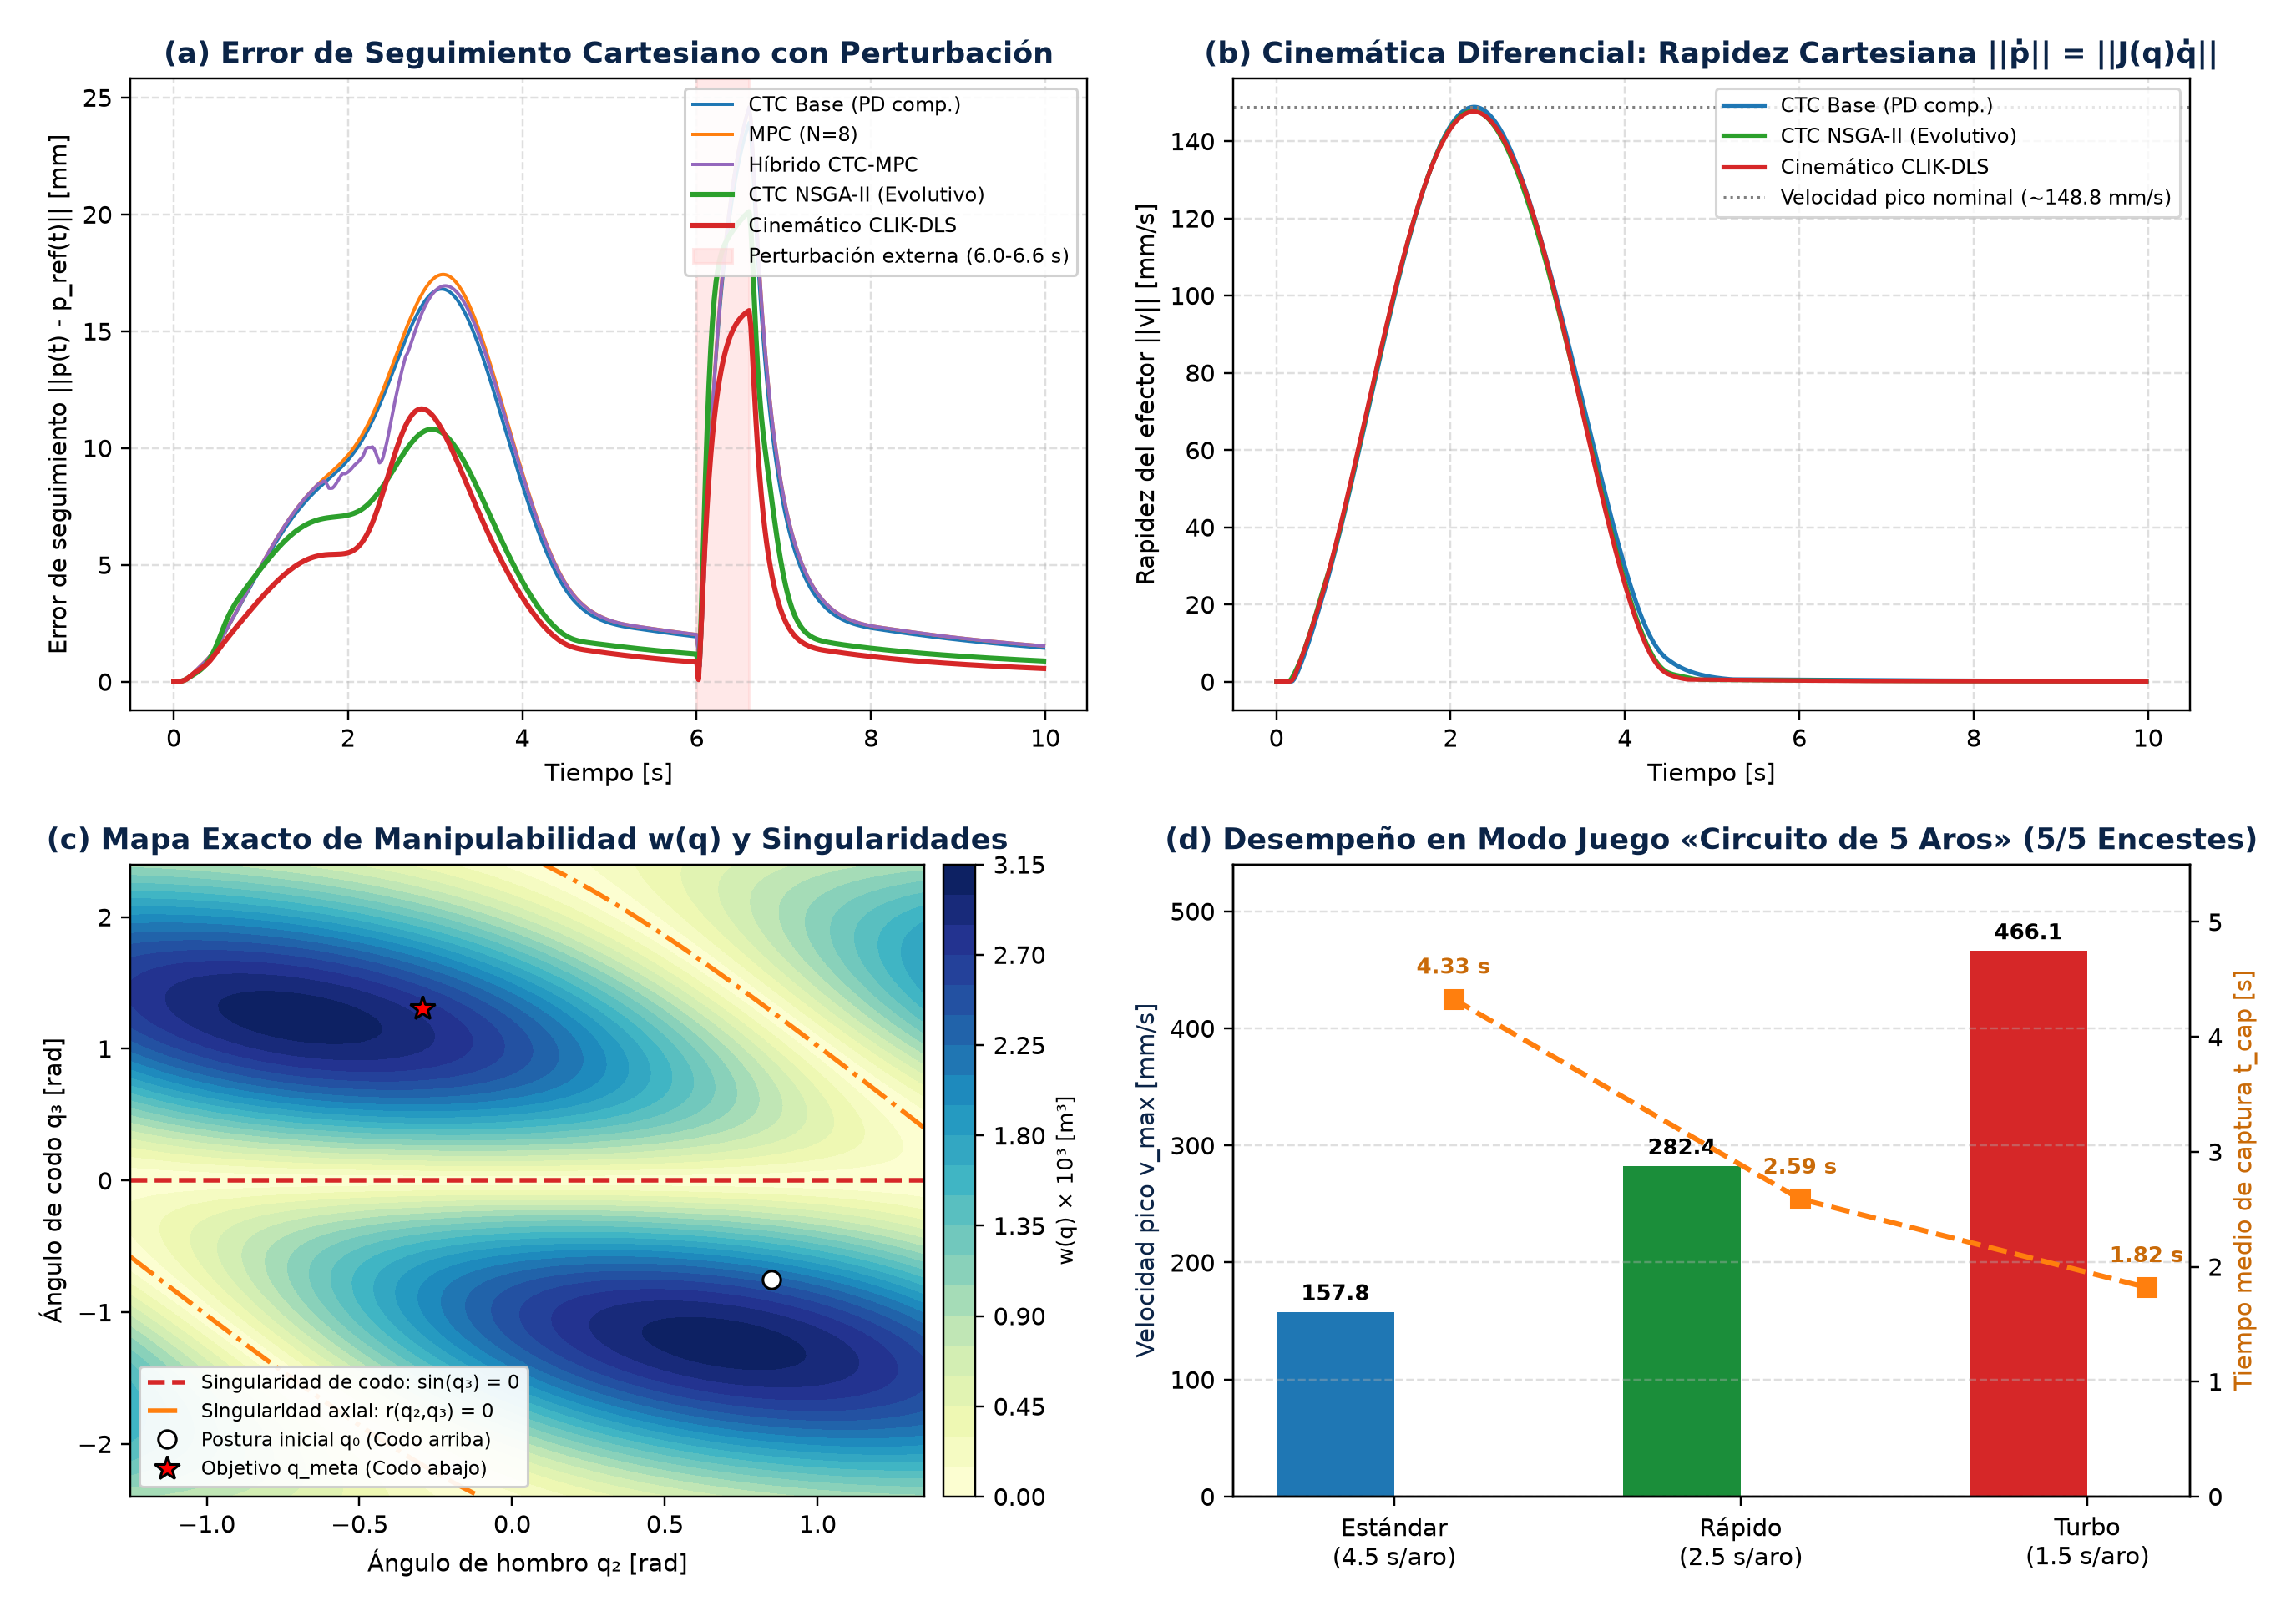
\includegraphics[width=1.08\textwidth]{results/figuras_examen_parcial/fig_curvas_simulacion.png}
\caption{Resultados experimentales de simulación: (a) evolución del error de seguimiento cartesiano ante perturbación externa para los 5 controladores; (b) perfil de rapidez cartesiana $\norm{\pdot}=\norm{J_{v}(\bm{q})\qdot}$; (c) mapa cuantitativo exacto del índice de manipulabilidad de Yoshikawa $w(q_{2},q_{3})$ mostrando las fronteras de singularidad de codo ($\sin q_{3}=0$) y axial de hombro ($r=0$); (d) velocidad pico y tiempo de captura en el Circuito de 5 Aros.}
\label{fig:curvas}
\end{figure}

\begin{cajaidea}[Interpretación física y cuantitativa de los resultados]
\begin{enumerate}[leftmargin=*, topsep=2pt, itemsep=1pt]
\item \textbf{Superioridad del Control Cinemático Amortiguado (KIN / CLIK-DLS):} Al realimentar directamente el error en el espacio de tarea cartesiano a través de $\Jdls(\bm{q})$, alcanza el menor error final ($0{,}273\;\text{mm}$ nominal y $0{,}565\;\text{mm}$ perturbado), el menor tiempo de captura ($4{,}38\;\text{s}$) y la recuperación más veloz tras la perturbación ($t_{\text{rec}}=0{,}242\;\text{s}$).
\item \textbf{Ganancia Evolutiva del CTC NSGA-II (EVO):} Reduce en $33{,}5\,\%$ el RMSE de seguimiento y en $42{,}2\,\%$ el error estacionario respecto al CTC base, acortando el tiempo de captura en $1{,}34\;\text{s}$ y el tiempo de recuperación ante perturbaciones en $34{,}4\,\%$ ($0{,}382\;\text{s}$ vs.\ $0{,}582\;\text{s}$) con menor consumo de energía de actuación ($0{,}4817\;\text{N}^{2}\text{m}^{2}\text{s}$).
\item \textbf{Aporte del Híbrido CTC--MPC (HYB):} Mejora el seguimiento transitorio respecto al MPC clásico ($6{,}815\;\text{mm}$ vs.\ $7{,}137\;\text{mm}$) garantizando $0\,\%$ de saturación de actuadores en todo el horizonte.
\end{enumerate}
\end{cajaidea}

% ---------------------------------------------------------------------
\subsection{Aplicación funcional: Modo Juego «Circuito de 5 Aros (Encestar Bola)» y Cambio de Estado Visual 3D}
\label{sec:game}
% ---------------------------------------------------------------------

Desde el punto de vista de la teoría de mecanismos, un manipulador RRR de 3\,GDL sin muñeca esférica controla los 3 grados de libertad traslacionales de la punta $\bm{p}=[x,y,z]\T\in\Real^{3}$, mientras que un lanzamiento parabólico libre requeriría al menos 5\,GDL más un actuador de apertura rápida para imponer independientemente el vector de velocidad de salida. Por ello, la tarea de encestar una esfera en aros distribuidos en el espacio 3D (\emph{inserción directa / dunk}) y la tarea de posicionar un foco/lente óptico sobre objetivos puntuales son físicamente rigurosas y aprovechan íntegramente la cinemática del robot.

En los módulos \texttt{main.py} y \texttt{models/brazo\_3d.xml} se implementó una esfera energética sin masa entre las mordazas de la pinza (\texttt{bola\_efector}) y un aro receptor (\texttt{objetivo\_aro\_base}) acoplados a una máquina de estados en tiempo real (Figura~\ref{fig:estados3d}) y tres perfiles de rapidez seleccionables (Tabla~\ref{tab:aros}):
\begin{itemize}[leftmargin=*, topsep=2pt, itemsep=1pt]
\item \textbf{ESPERANDO ORDEN (Azul Cian):} manipulador estabilizado a la espera de una coordenada XYZ o del inicio del circuito competitivo.
\item \textbf{EN MOVIMIENTO (Esfera Naranja $\to$ Aro Rojo):} el brazo ejecuta la trayectoria hacia el aro objetivo midiendo en vivo la rapidez cartesiana $\norm{\bm{v}}=\norm{J_{v}(\bm{q})\,\qdot}$ y actualizando el registro de velocidad pico $v_{\max}$.
\item \textbf{PERTURBACIÓN ACTIVA (Esfera Magenta):} señaliza visualmente la acción de fuerzas externas sobre las articulaciones y la respuesta correctiva del controlador activo.
\item \textbf{¡ENCESTADO / OBJETIVO ALCANZADO! (Verde Esmeralda):} en el instante en que $\norm{\bm{p}(t)-\bm{p}_{\text{obj}}}<2{,}0\;\text{mm}$, tanto la esfera del efector como el aro objetivo conmutan a color \textbf{Verde Esmeralda brillante} en la escena 3D de MuJoCo, se congela el tiempo de captura $t_{\text{cap}}$, se incrementa el marcador de encestes y, en modo juego, el robot avanza automáticamente hacia el siguiente aro hasta completar el circuito de 5/5 objetivos.
\end{itemize}

\begin{figure}[htbp]
\centering
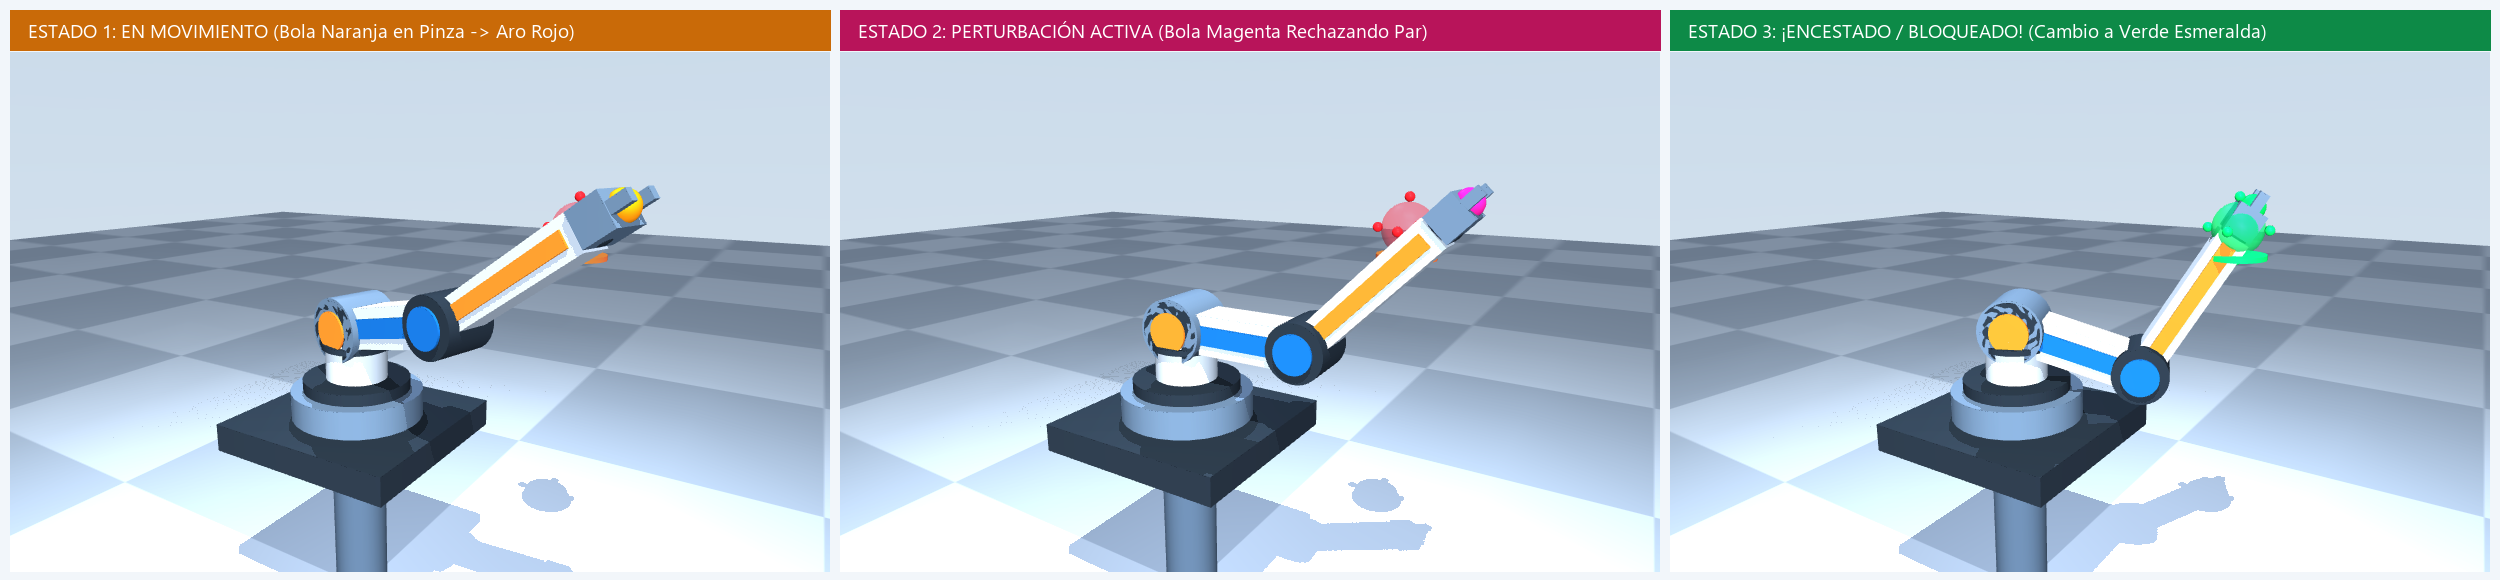
\includegraphics[width=0.99\textwidth]{results/figuras_examen_parcial/fig_estados_3d_enceste.png}
\caption{Capturas reales del Gemelo Digital 3D en MuJoCo (\texttt{main.py}) demostrando la transición automática de estado visual del robot: (izquierda) Estado 1 \emph{EN MOVIMIENTO} con esfera naranja entre las mordazas de la pinza aproximándose al aro rojo; (centro) Estado 2 \emph{PERTURBACIÓN ACTIVA} con esfera en magenta; (derecha) Estado 3 \emph{¡ENCESTADO / BLOQUEADO!} donde la esfera y el aro conmutan a verde esmeralda al ingresar en la tolerancia de $<2{,}0\;\text{mm}$.}
\label{fig:estados3d}
\end{figure}

\begin{table}[htbp]
\centering
\caption{Métricas experimentales del Modo Juego «Circuito de 5 Aros» en los tres perfiles de rapidez.}\label{tab:aros}
\footnotesize
\setlength{\tabcolsep}{5pt}
\begin{tabular}{lcccccc}
\toprule
\textbf{Perfil} & \textbf{Duración/aro} & \textbf{Aros encestados} & $t_{\text{cap}}$ \textbf{medio} & $v_{\max}$ \textbf{pico} & \textbf{Rapidez media} & \textbf{Energía total} \\
 & {[s]} & & {[s]} & {[mm/s]} & {[mm/s]} & {[$\text{N}^{2}\text{m}^{2}\text{s}$]} \\
\midrule
Estándar & 4{,}5 & \textbf{5/5} & 4{,}33 & 157{,}8 &  52{,}5 & 1{,}1200 \\
Rápido   & 2{,}5 & \textbf{5/5} & 2{,}59 & 282{,}4 &  87{,}0 & 0{,}6830 \\
Turbo    & 1{,}5 & \textbf{5/5} & 1{,}82 & \textbf{466{,}1} & 130{,}6 & 0{,}4670 \\
\bottomrule
\end{tabular}
\end{table}

% =====================================================================
\section{Opinión personal y apreciación crítica}
% =====================================================================

El desarrollo integral de este Trabajo Parcial ha permitido comprobar que el dominio de la robótica moderna exige articular tres pilares indivisibles: el rigor geométrico-algebraico (transformaciones de Denavit-Hartenberg, cinemática inversa cerrada y estructura del Jacobiano lineal y angular), el análisis estructural de las singularidades y la validación sobre un motor físico realista sujeto a límites de torque. La experiencia de implementar el mismo manipulador antropomórfico de 3\,GDL tanto en scripts simbólicos y numéricos de MATLAB como en el gemelo digital 3D en MuJoCo evidenció que los fenómenos críticos de operación ---como la pérdida de rango en $\sin q_{3}=0$ al conmutar entre configuraciones de codo arriba y codo abajo--- no pueden resolverse únicamente con ganancias estáticas, sino que requieren regularización diferencial amortiguada (CLIK-DLS) y sintonización multiobjetivo (NSGA-II). Asimismo, la incorporación del modo interactivo de enceste con retroalimentación visual de estado demuestra cómo los indicadores cinemáticos ($\norm{\pdot}$, $v_{\max}$, $w(\bm{q})$) cobran pleno sentido ingenieril cuando se traducen en métricas de misión observables en tiempo real.

% =====================================================================
\section{Conclusiones}
% =====================================================================

\begin{enumerate}[leftmargin=*, topsep=3pt, itemsep=3pt]
\item Se formuló, implementó y verificó con discrepancia numérica inferior a $10^{-16}\;\text{m}$ la cinemática directa del manipulador antropomórfico RRR de 3\,GDL (Conejo Benítez, 2021) mediante los métodos geométrico, de transformaciones homogéneas sucesivas y de Denavit-Hartenberg, así como su cinemática inversa analítica en ambas ramas (codo abajo y codo arriba).

\item Se dedujo el Jacobiano geométrico completo $6\times 3$, compuesto por el bloque traslacional $J_{v}(\bm{q})$ y el bloque rotacional $J_{\omega}(\bm{q})=[\bm{z}_{0}\;\;\bm{z}_{1}\;\;\bm{z}_{2}]$, demostrando la factorización exacta $\det J_{v}(\bm{q})=-L_{1}L_{2}\sin q_{3}\,\bigl(L_{1}\cos q_{2}+L_{2}\cos(q_{2}+q_{3})\bigr)$, la cual caracteriza de forma cerrada las singularidades de codo ($q_{3}=0,\pm\pi$) y axial de hombro ($r=0$).

\item El controlador cinemático en lazo cerrado con pseudoinversa amortiguada de Levenberg--Marquardt (\textbf{CLIK-DLS}) alcanzó las mejores prestaciones globales del estudio: error estacionario de $0{,}273\;\text{mm}$ en régimen nominal ($0{,}565\;\text{mm}$ bajo perturbación), tiempo de captura de $4{,}38\;\text{s}$ y tiempo de recuperación tras perturbación de tan solo $0{,}242\;\text{s}$.

\item La sintonización evolutiva multiobjetivo mediante \textbf{NSGA-II} del controlador por torque computado (\textbf{CTC NSGA-II}) logró dominar simultáneamente al controlador CTC base en precisión y esfuerzo energético, reduciendo el RMSE de seguimiento en $33{,}5\,\%$ (de $6{,}879\;\text{mm}$ a $4{,}573\;\text{mm}$) y el error final en $42{,}2\,\%$ (de $0{,}892\;\text{mm}$ a $0{,}516\;\text{mm}$).

\item La máquina de estados 3D y el \textbf{Modo Juego «Circuito de 5 Aros»} permitieron validar la operación continua del robot en tres regímenes de rapidez, completando el $100\,\%$ de los encestes ($5/5$ aros con error $<2{,}0\;\text{mm}$) y alcanzando velocidades cartesianas pico desde $157{,}8\;\text{mm/s}$ (modo Estándar) hasta $466{,}1\;\text{mm/s}$ (modo Turbo).
\end{enumerate}

% =====================================================================
\section{Recomendaciones}
% =====================================================================

\begin{enumerate}[leftmargin=*, topsep=3pt, itemsep=3pt]
\item Para la implementación sobre el banco experimental físico con servomotores Dynamixel AX-18A y AX-12A, se recomienda incorporar un filtro pasa-bajas de segundo orden (o un observador de estado tipo Kalman) en el cálculo de $\qdot$ a fin de mitigar el ruido de cuantización de los encoders antes de multiplicar por la ganancia derivativa $K_{d}$.

\item Adoptar el perfil \textbf{Rápido ($2{,}5\;\text{s/aro}$)} combinado con los controladores \textbf{CLIK-DLS} o \textbf{CTC NSGA-II} como régimen nominal de trabajo en tareas de captura repetitiva, dado que garantiza el $100\,\%$ de encestes ($t_{\text{cap}}=2{,}59\;\text{s}$, $v_{\max}=282{,}4\;\text{mm/s}$) reduciendo el esfuerzo energético acumulado en un $39{,}0\,\%$ respecto al régimen estándar.

\item En aplicaciones futuras que demanden desacoplar la orientación de la herramienta respecto de la posición $(x,y,z)$ (por ejemplo, inspección óptica con ángulo de incidencia variable o manipulación con pinza orientada), ampliar la cadena cinemática de 3\,GDL a 6\,GDL agregando una muñeca esférica de ejes concurrentes ($\text{R--R--R}$).

\item Mantener activo el amortiguamiento adaptativo $\lambda\in[0{,}015,\,0{,}025]$ en la pseudoinversa DLS siempre que se planifiquen trayectorias cartesianas que obliguen al codo a conmutar de signo ($q_{3}<0\leftrightarrow q_{3}>0$).
\end{enumerate}

% =====================================================================
% 6. REFERENCIAS BIBLIOGRÁFICAS (FORMATO APA 7.ª EDICIÓN, SIN TÍTULO DUPLICADO)
% =====================================================================
\section{Referencias bibliográficas (Norma APA 7.ª ed.)}
\begingroup
\setlength{\parindent}{-1.8em}
\setlength{\leftskip}{1.8em}
\setlength{\parskip}{6pt}

Barrientos, A., Peñín, L.~F., Balaguer, C., \& Aracil, R. (2007). \emph{Fundamentos de robótica} (2.ª~ed.). McGraw-Hill Interamericana.

Conejo Benítez, C.~E. (2021). \emph{Modelado y control de un brazo robótico de 3 grados de libertad} [Tesis de maestría, Universidad de Guanajuato]. Repositorio Institucional de la Universidad de Guanajuato.

Craig, J.~J. (2018). \emph{Introduction to robotics: Mechanics and control} (4th~ed.). Pearson.

Deb, K., Pratap, A., Agarwal, S., \& Meyarivan, T. (2002). A fast and elitist multiobjective genetic algorithm: NSGA-II. \emph{IEEE Transactions on Evolutionary Computation}, \emph{6}(2), 182--197. \url{https://doi.org/10.1109/4235.996017}

Siciliano, B., Sciavicco, L., Villani, L., \& Oriolo, G. (2009). \emph{Robotics: Modelling, planning and control}. Springer. \url{https://doi.org/10.1007/978-1-84628-642-1}

Todorov, E., Erez, T., \& Tassa, Y. (2012). MuJoCo: A physics engine for model-based control. En \emph{Proceedings of the 2012 IEEE/RSJ International Conference on Intelligent Robots and Systems (IROS)} (pp.~5026--5033). IEEE. \url{https://doi.org/10.1109/IROS.2012.6386109}

Yoshikawa, T. (1985). Manipulability of robotic mechanisms. \emph{The International Journal of Robotics Research}, \emph{4}(2), 3--9. \url{https://doi.org/10.1177/027836498500400201}

\endgroup

\clearpage
% =====================================================================
\section{Anexos: esquemas realizados y verificación del sistema}
% =====================================================================

% ---------------------------------------------------------------------
\subsection{Anexo A --- Esquema de la arquitectura de control multimodo y máquina de estados}
% ---------------------------------------------------------------------

\begin{figure}[!htb]
\centering
\resizebox{0.96\textwidth}{!}{%
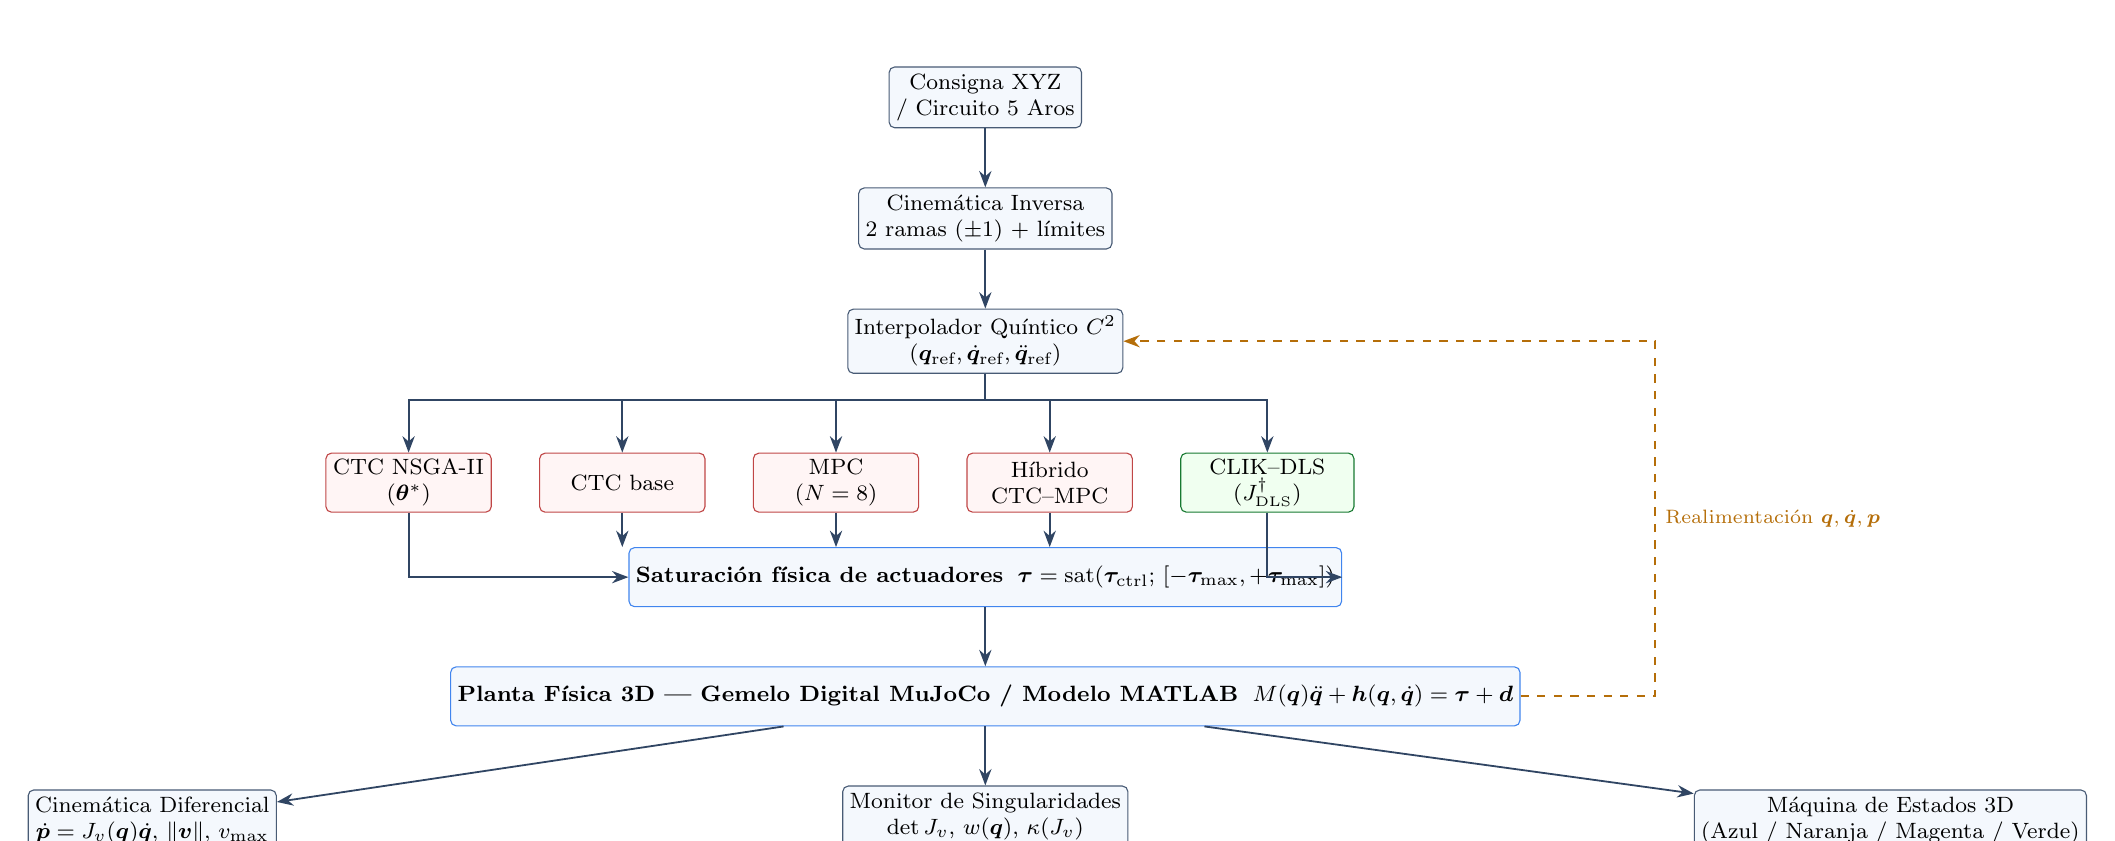
\begin{tikzpicture}[>=Stealth, scale=0.95, font=\footnotesize,
  node distance=7.5mm and 12mm,
  block/.style={rectangle, draw=uniAzul!75, fill=cajaBg, rounded corners=2pt,
                minimum width=24mm, minimum height=7.5mm, align=center, inner sep=2.5pt},
  bigblock/.style={rectangle, draw=uniAzulC!85, fill=cajaBg, rounded corners=2pt,
                minimum width=76mm, minimum height=7.5mm, align=center, inner sep=2.5pt},
  ctrl/.style={rectangle, draw=uniRojo!80, fill=red!4, rounded corners=2pt,
                minimum width=21mm, minimum height=7.5mm, align=center, inner sep=2pt},
  ctrlkin/.style={rectangle, draw=verdeOk!85!black, fill=green!6, rounded corners=2pt,
                minimum width=22mm, minimum height=7.5mm, align=center, inner sep=2pt},
  arr/.style={->, line width=0.65pt, color=uniAzul!85}]

\node[block] (cmd) {Consigna XYZ \\ / Circuito 5 Aros};
\node[block, below=of cmd] (ik) {Cinemática Inversa \\ 2 ramas ($\pm 1$) + límites};
\node[block, below=of ik] (ref) {Interpolador Quíntico $C^{2}$ \\ ($\bm{q}_{\text{ref}},\qdot_{\text{ref}},\qddot_{\text{ref}}$)};

\node[ctrl, below left=10mm and 18mm of ref] (ctc) {CTC base};
\node[ctrl, left=6mm of ctc] (evo) {CTC NSGA-II \\ ($\bm{\theta}^{*}$)};
\node[ctrl, right=6mm of ctc] (mpc) {MPC \\ ($N=8$)};
\node[ctrl, right=6mm of mpc] (hyb) {Híbrido \\ CTC--MPC};
\node[ctrlkin, right=6mm of hyb] (kin) {CLIK--DLS \\ ($\Jdls$)};

\node[bigblock, below=22mm of ref] (sat) {\textbf{Saturación física de actuadores} $\;\bm{\tau}=\operatorname{sat}(\bm{\tau}_{\text{ctrl}};\,[-\bm{\tau}_{\max},+\bm{\tau}_{\max}])$};
\node[bigblock, below=of sat] (plant) {\textbf{Planta Física 3D --- Gemelo Digital MuJoCo / Modelo MATLAB} $\;M(\bm{q})\qddot+\bm{h}(\bm{q},\qdot)=\bm{\tau}+\bm{d}$};

\node[block, below left=8mm and 22mm of plant] (jac) {Cinemática Diferencial \\ $\pdot=J_{v}(\bm{q})\qdot$, $\norm{\bm{v}}$, $v_{\max}$};
\node[block, below=of plant] (sing) {Monitor de Singularidades \\ $\det J_{v},\,w(\bm{q}),\,\kappa(J_{v})$};
\node[block, below right=8mm and 22mm of plant] (state) {Máquina de Estados 3D \\ (Azul / Naranja / Magenta / Verde)};

\draw[arr] (cmd) -- (ik);
\draw[arr] (ik) -- (ref);
\draw[arr] (ref.south) -- ++(0,-3.5mm) -| (evo.north);
\draw[arr] (ref.south) -- ++(0,-3.5mm) -| (ctc.north);
\draw[arr] (ref.south) -- ++(0,-3.5mm) -| (mpc.north);
\draw[arr] (ref.south) -- ++(0,-3.5mm) -| (hyb.north);
\draw[arr] (ref.south) -- ++(0,-3.5mm) -| (kin.north);
\draw[arr] (evo.south) |- (sat.west);
\draw[arr] (ctc.south) -- (ctc.south |- sat.north);
\draw[arr] (mpc.south) -- (mpc.south |- sat.north);
\draw[arr] (hyb.south) -- (hyb.south |- sat.north);
\draw[arr] (kin.south) |- (sat.east);
\draw[arr] (sat) -- (plant);
\draw[arr] (plant) -- (jac);
\draw[arr] (plant) -- (sing);
\draw[arr] (plant) -- (state);
\draw[arr, dashed, color=naranja!90!black] (plant.east) -- ++(18mm,0) |- node[pos=0.25, right, font=\scriptsize] {Realimentación $\bm{q},\qdot,\bm{p}$} (ref.east);
\end{tikzpicture}}%
\caption{Esquema general de la arquitectura de control multimodo y máquina de estados del robot antropomórfico de 3\,GDL implementada en \texttt{main.py} y \texttt{matlab/simulacion\_3gdl\_examen\_parcial.m}.}
\label{fig:arquitectura}
\end{figure}

% ---------------------------------------------------------------------
\subsection{Anexo B --- Implementación en MATLAB de Cinemática DH, Jacobiano y Control CLIK-DLS}
% ---------------------------------------------------------------------

\begin{lstlisting}[caption={Funciones principales de Denavit-Hartenberg, Jacobiano geométrico $6\times 3$ y ley de control cinemático CLIK-DLS en \texttt{matlab/simulacion\_3gdl\_examen\_parcial.m}.},label={lst:clik}]
function [p, T01, T02, T03] = fk_dh_3gdl(q, robot)
    A1 = dh_mat(q(1), robot.d1, 0,        pi/2);
    A2 = dh_mat(q(2), 0,        robot.L1, 0);
    A3 = dh_mat(q(3), 0,        robot.L2, 0);
    T01 = A1;  T02 = T01 * A2;  T03 = T02 * A3;
    p = T03(1:3, 4);
end

function [Jv, Jw, J_full, detJ, w_yosh] = jacobiano_3gdl(q, robot)
    [~, T01, T02, ~] = fk_dh_3gdl(q, robot);
    r   = robot.L1 * cos(q(2)) + robot.L2 * cos(q(2) + q(3));
    drb = -robot.L1 * sin(q(2)) - robot.L2 * sin(q(2) + q(3));
    drc = -robot.L2 * sin(q(2) + q(3));
    Jv  = [-r*sin(q(1)), drb*cos(q(1)), drc*cos(q(1));
            r*cos(q(1)), drb*sin(q(1)), drc*sin(q(1));
            0,           r,             robot.L2*cos(q(2)+q(3))];
    z0 = [0; 0; 1];  z1 = T01(1:3, 3);  z2 = T02(1:3, 3);
    Jw = [z0, z1, z2];
    J_full = [Jv; Jw];
    detJ = -robot.L1 * robot.L2 * sin(q(3)) * r;
    w_yosh = abs(detJ);
end

function dq_cmd = clik_dls(q, dq_ref, p_des, p_now, robot, lambda, K_cart)
    [Jv, ~, ~, ~, ~] = jacobiano_3gdl(q, robot);
    J_dls  = Jv' / (Jv * Jv' + (lambda^2) * eye(3));
    dq_cmd = dq_ref + J_dls * (K_cart * (p_des - p_now));
end
\end{lstlisting}
\clearpage  % Fuerza al Anexo C a empezar en una nueva página
% ---------------------------------------------------------------------
\subsection{Anexo C --- Verificación algebraica y numérica de las matrices homogéneas acumuladas}
% ---------------------------------------------------------------------

\begin{table}[!htbp]
\centering
\caption{Expresión simbólica y evaluación numérica exacta de los vectores de posición de las matrices homogéneas acumuladas $T_{0}^{1}$, $T_{0}^{2}$ y $T_{0}^{3}$ en la postura inicial $\bm{q}_{0}=[-1{,}10,\;0{,}85,\;-0{,}75]\T\;\text{rad}$ ($d_{1}=0{,}079\;\text{m}$, $L_{1}=0{,}113\;\text{m}$, $L_{2}=0{,}140\;\text{m}$).}\label{tab:verif}
\footnotesize
\setlength{\tabcolsep}{4pt}
\begin{tabular}{c l l}
\toprule
\textbf{Matriz} & \textbf{Expresión analítica de la columna de posición} $\bm{p}_{i}(\bm{q})$ & \textbf{Evaluación en} $\bm{q}_{0}$ {[m]} \\
\midrule
$T_{0}^{1}(1:3,4)$ & $[0,\;0,\;d_{1}]\T$ & $[0{,}000000,\;0{,}000000,\;0{,}079000]\T$ \\[3pt]
$T_{0}^{2}(1:3,4)$ & $[L_{1}\cos q_{2}\cos q_{1},\;L_{1}\cos q_{2}\sin q_{1},\;d_{1}+L_{1}\sin q_{2}]\T$ & $[0{,}033828,\;-0{,}066465,\;0{,}163895]\T$ \\[3pt]
$T_{0}^{3}(1:3,4)$ & $\bigl[(L_{1}c_{2}+L_{2}c_{23})\cos q_{1},\;(L_{1}c_{2}+L_{2}c_{23})\sin q_{1},\;d_{1}+L_{1}s_{2}+L_{2}s_{23}\bigr]\T$ & $[0{,}097015,\;-0{,}190610,\;0{,}177871]\T$ \\
\bottomrule
\end{tabular}
\end{table}

\end{document}
